\section{模型：持续状态架构}\label{sec:model}

\subsection{整体结构（byte 级语言模型 + 有状态核心）}\label{sec:model-overall}

模型由两部分组成。

\textbf{（1）byte 级语言模型。}分词单位是\textbf{字节}而不是词：ByteTokenizer 直接以 UTF-8 字节为 token，
词表大小 300（256 个字节值 $+$ \texttt{pad}=256 $+$ \texttt{eos}=257）。
好处是不存在词表外的「词」，任何文本都能无损进出；损失以 \textbf{bits/byte} 计，
跨语言、跨编码格式可比——这就是主指标口径的来源（\S\ref{sec:metric}）。

\textbf{（2）有状态核心。}一次前向吃一个 64 字节的 patch（记 $B=64$）：
\begin{equation}
\mathrm{logits},\; \mathrm{state} = \mathrm{model}(x,\ \mathrm{state},\ \mathit{lock\_mem}),
\qquad x \in \mathbb{Z}_B^{1\times 64},
\label{eq:model-call}
\end{equation}
上下文的延续不靠 KV cache 累积，靠 $s' = f(x,s)$ 在 patch 之间递归传递（式 \eqref{eq:forward}）。
注意力只在\textbf{当前 patch 片内}做局部混合，跨 patch 的历史一律由状态携带——
这就是「有状态」的准确含义：历史信息的唯一通道是状态。

图 \ref{fig:arch} 给出整体结构与原语的对应关系。正式配置为 \texttt{GRIDMAN\_MEDIUM}：
\texttt{embed\_dim}=1024、\texttt{blocks}=3（对应 4 个 \texttt{c\_state}）、
\texttt{patch\_size}=64，模型参数 437.8M\footnote{配置与参数量引自团队内部文档《论文大纲-B》第 0 章与配图；
代码事实对应实现仓 \texttt{zhihumomo/ouro-research}。}。

\textbf{实现版本声明（重要）。}本文所有实验数字来自 \texttt{v\_0d3} 检查点；
模型行为的描述以 \texttt{v\_0d4} 实现（2026-10-18 更新）为准。两版差异集中在
\texttt{memory} 的作用域与训练配置，见表 \ref{tab:version}。
差异不影响本文的推理侧结论：所有评测都在 $\mathrm{batch}=1$ 上进行，
v\_0d4 的序列级记忆在 $\mathrm{batch}=1$ 时读写单个槽位，与 v\_0d3 的
\texttt{[1,\ldots]} 布局逐位对应（\S\ref{sec:train}）。

\begin{table}[H]
\centering
\caption{实现版本差异（v\_0d3 $\to$ v\_0d4）。本文检查点由 v\_0d3 训练产生；行为描述以 v\_0d4 为准。}
\label{tab:version}
\footnotesize
\begin{tabularx}{\linewidth}{@{}l X X@{}}
\toprule
项 & v\_0d3（本文检查点） & v\_0d4（现行实现） \\
\midrule
\texttt{memory} 作用域 & 跨样本共享（形状 $[1,\ldots]$） & \textbf{序列级私有槽位}（$[\mathrm{cap},\ldots]$，$\mathrm{cap}=\mathrm{max\_batch}$） \\
提交规则 & 跨 batch 求均值 & \textbf{无跨流平均}——序列间零泄漏 \\
跨卡同步 & 每 patch \texttt{all\_reduce} 均值 & \textbf{已删除}，记忆 rank 私有不通信 \\
写入门控偏置初始化 & $-6.0$ & $-\ln 63\approx-4.14$（对齐 $4096$-token 队列视界） \\
MEDIUM \texttt{chunk\_size} / \texttt{bptt} & $192$ / $4$ & $1$ / $16$ \\
存档格式 & \texttt{global\_memory} 顶层字段 & memory 移入 per-rank runtime\_states，\textbf{与 v\_0d3 存档不兼容} \\
\bottomrule
\end{tabularx}
\end{table}

\begin{figure}[t]
\centering
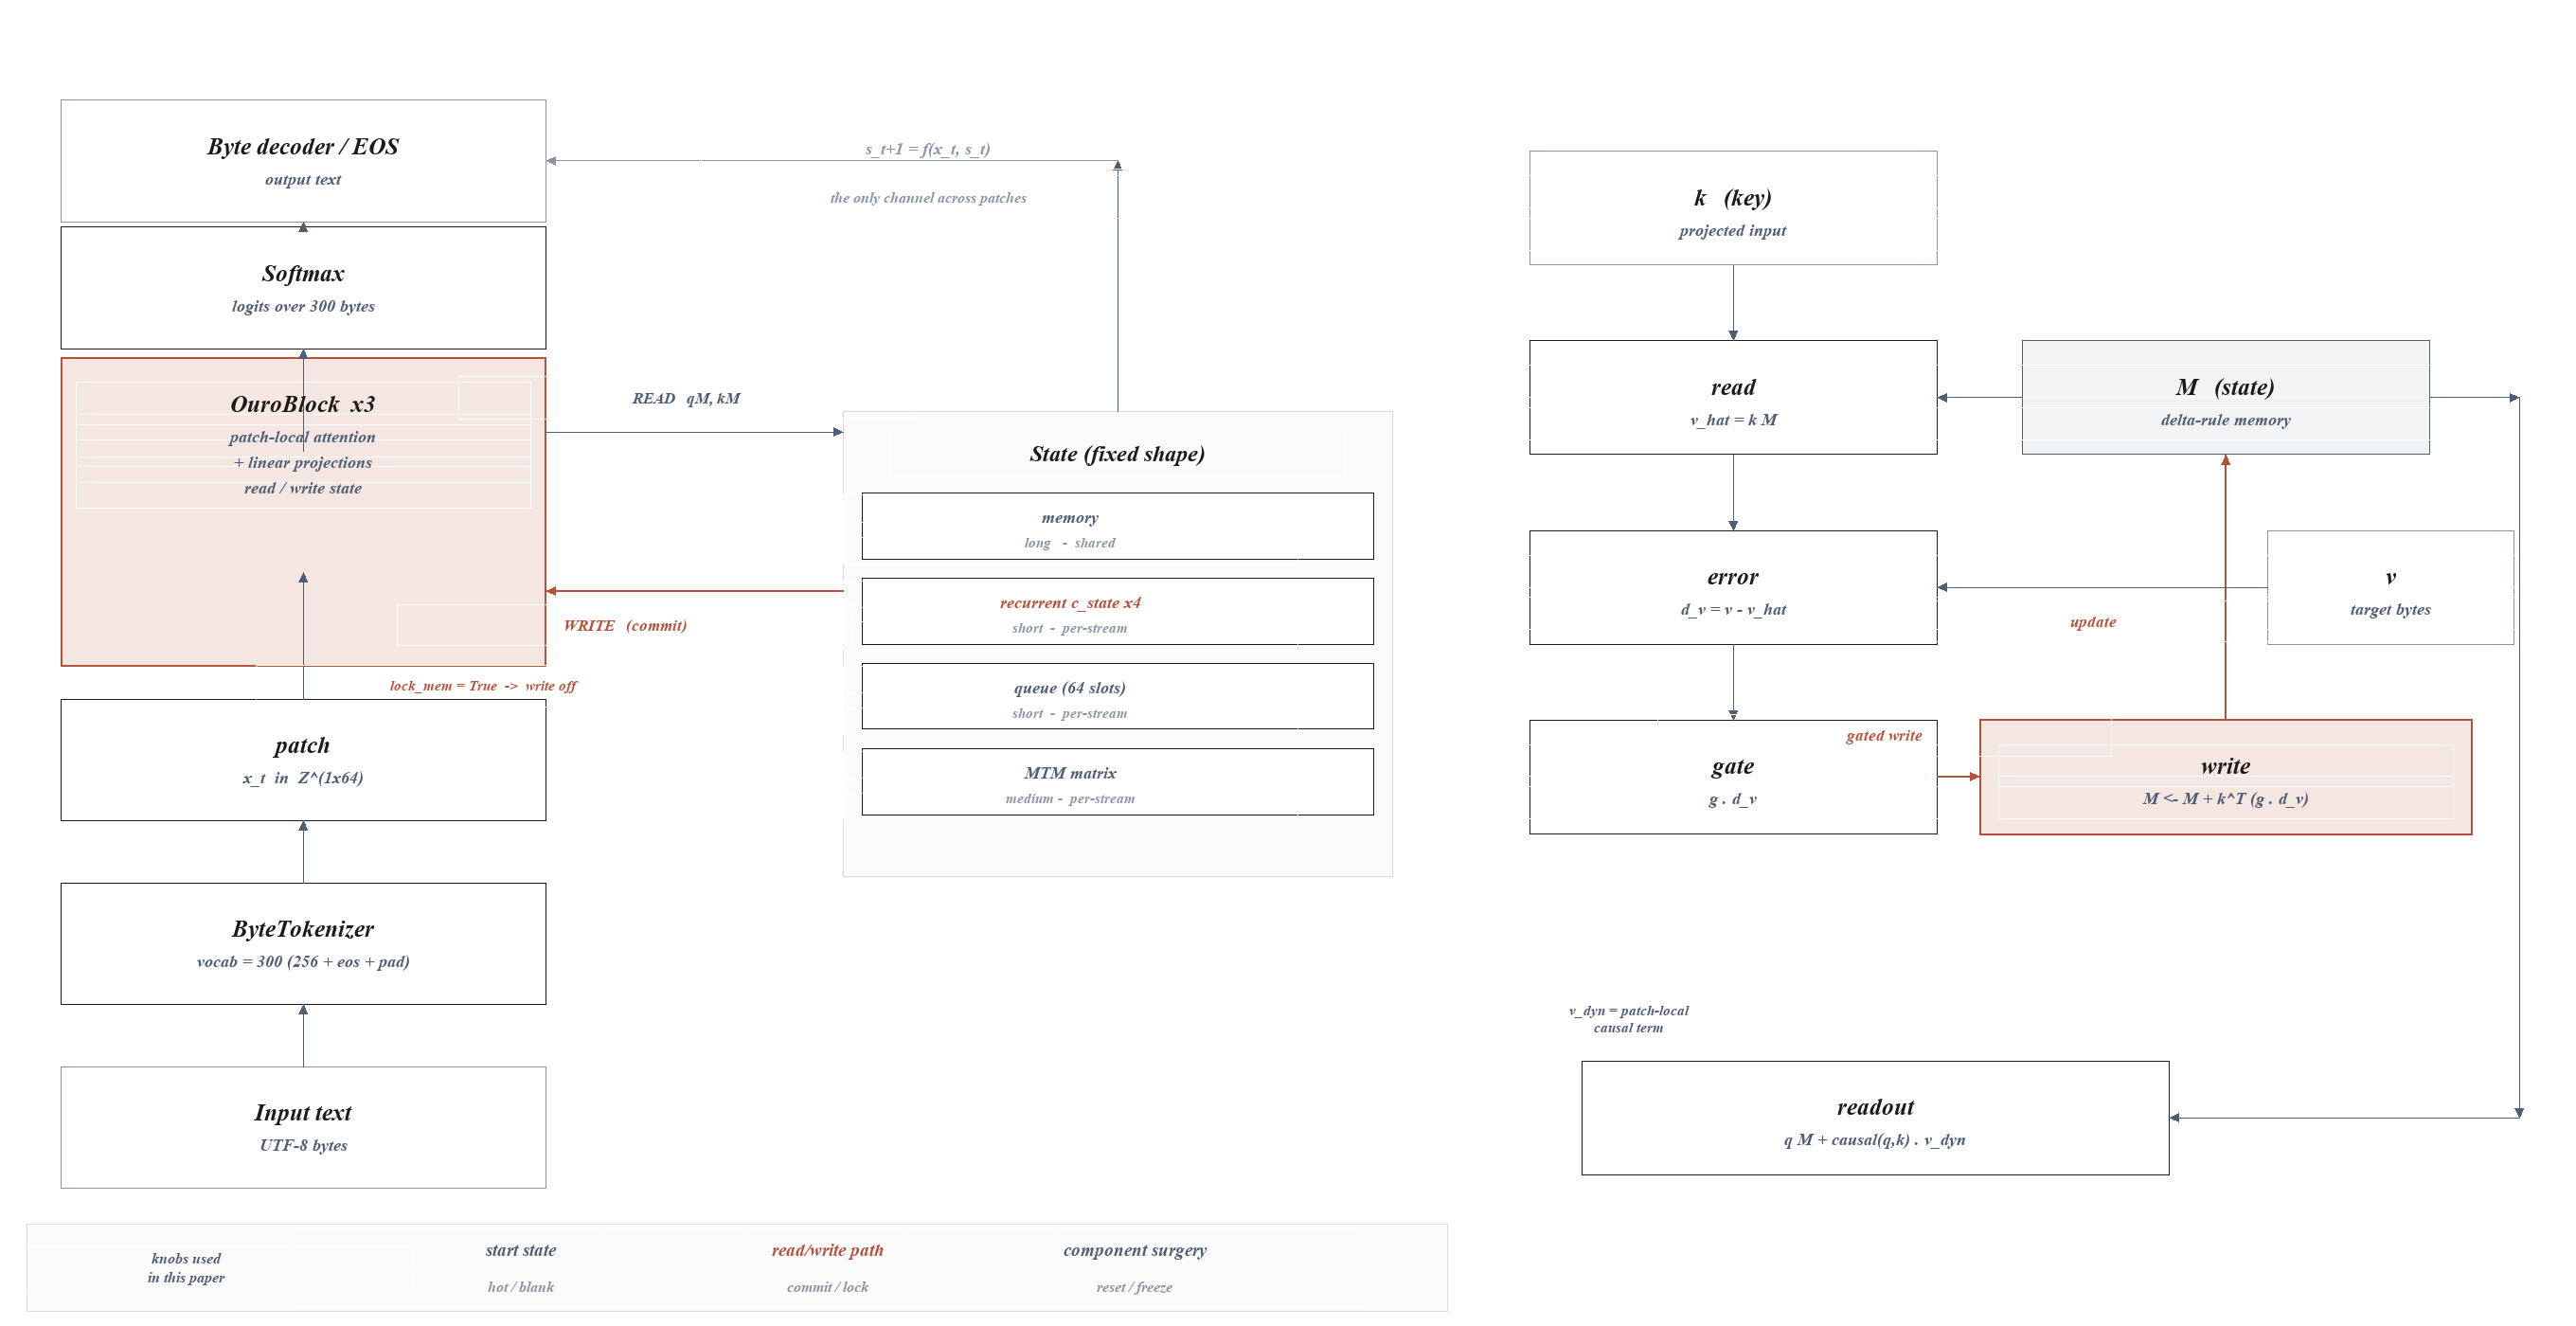
\includegraphics[width=\linewidth]{fig_arch.png}
\caption{持续状态架构与状态读写接口。左：一条跨 patch 的递归流——
输入文本经 byte 分词后在 patch 内做局部注意力混合，patch 之间的唯一信息通道是状态四件套；
右：原语 OuroCell 的读写链条（读出 $\hat v = kM$ $\to$ 误差 $\Delta v = v - \hat v$ $\to$ 门控写入
$M \leftarrow M + k^{\top}(g \cdot \Delta v)$ $\to$ 读出 $qM + \text{因果分数} \cdot v_{\mathrm{dyn}}$）。
下方给出本文实验用到的三类操纵旋钮：起点状态（热启动 / 空白）、读写路径（commit / $\mathit{lock}$）、
组件手术（重置 / 冻结）。本图由 Visio 绘制（源文件 \texttt{figs/fig\_arch.vsdx}，
用 VisioRender 渲染为 PNG；等价的矢量版本为 \texttt{figs/fig\_arch\_matplotlib.pdf}）。}
\label{fig:arch}
\end{figure}

\subsection{四件套状态及其作用域}\label{sec:model-state}

状态由四个分量构成，按时间尺度与作用域分工，见表 \ref{tab:state} 与图 \ref{fig:state-scales}。

\begin{table}[t]
\centering
\caption{状态四件套：机制、时间尺度与作用域。写入规则均为前向局部规则（无反向传播）。}
\label{tab:state}
\footnotesize
\begin{tabularx}{\linewidth}{@{}l X c X X@{}}
\toprule
分量 & 机制 & 时间尺度 & 作用域 & 写入规则 \\
\midrule
\texttt{memory} & delta 规则快权重矩阵（每层一块） & 长 & \textbf{序列级私有}（v\_0d4；v\_0d3 为跨样本共享、按流平均） & 误差驱动外积，恒等初始化 \\
\texttt{recurrent} & 块级循环状态 \texttt{c\_state}（$3+1$ 个） & 短 & 逐样本私有 & LSTM 式门控 cell \\
\texttt{queue} & 64 槽滚动队列 & 短 & 逐样本私有 & FIFO，存顶层 \texttt{c\_state} 历史 \\
\texttt{MTM} & 中期矩阵记忆 & 中 & 逐样本私有 & delta 规则，写入源为队列滑出的旧 \texttt{c\_state} \\
\bottomrule
\end{tabularx}
\end{table}

\begin{figure}[t]
\centering
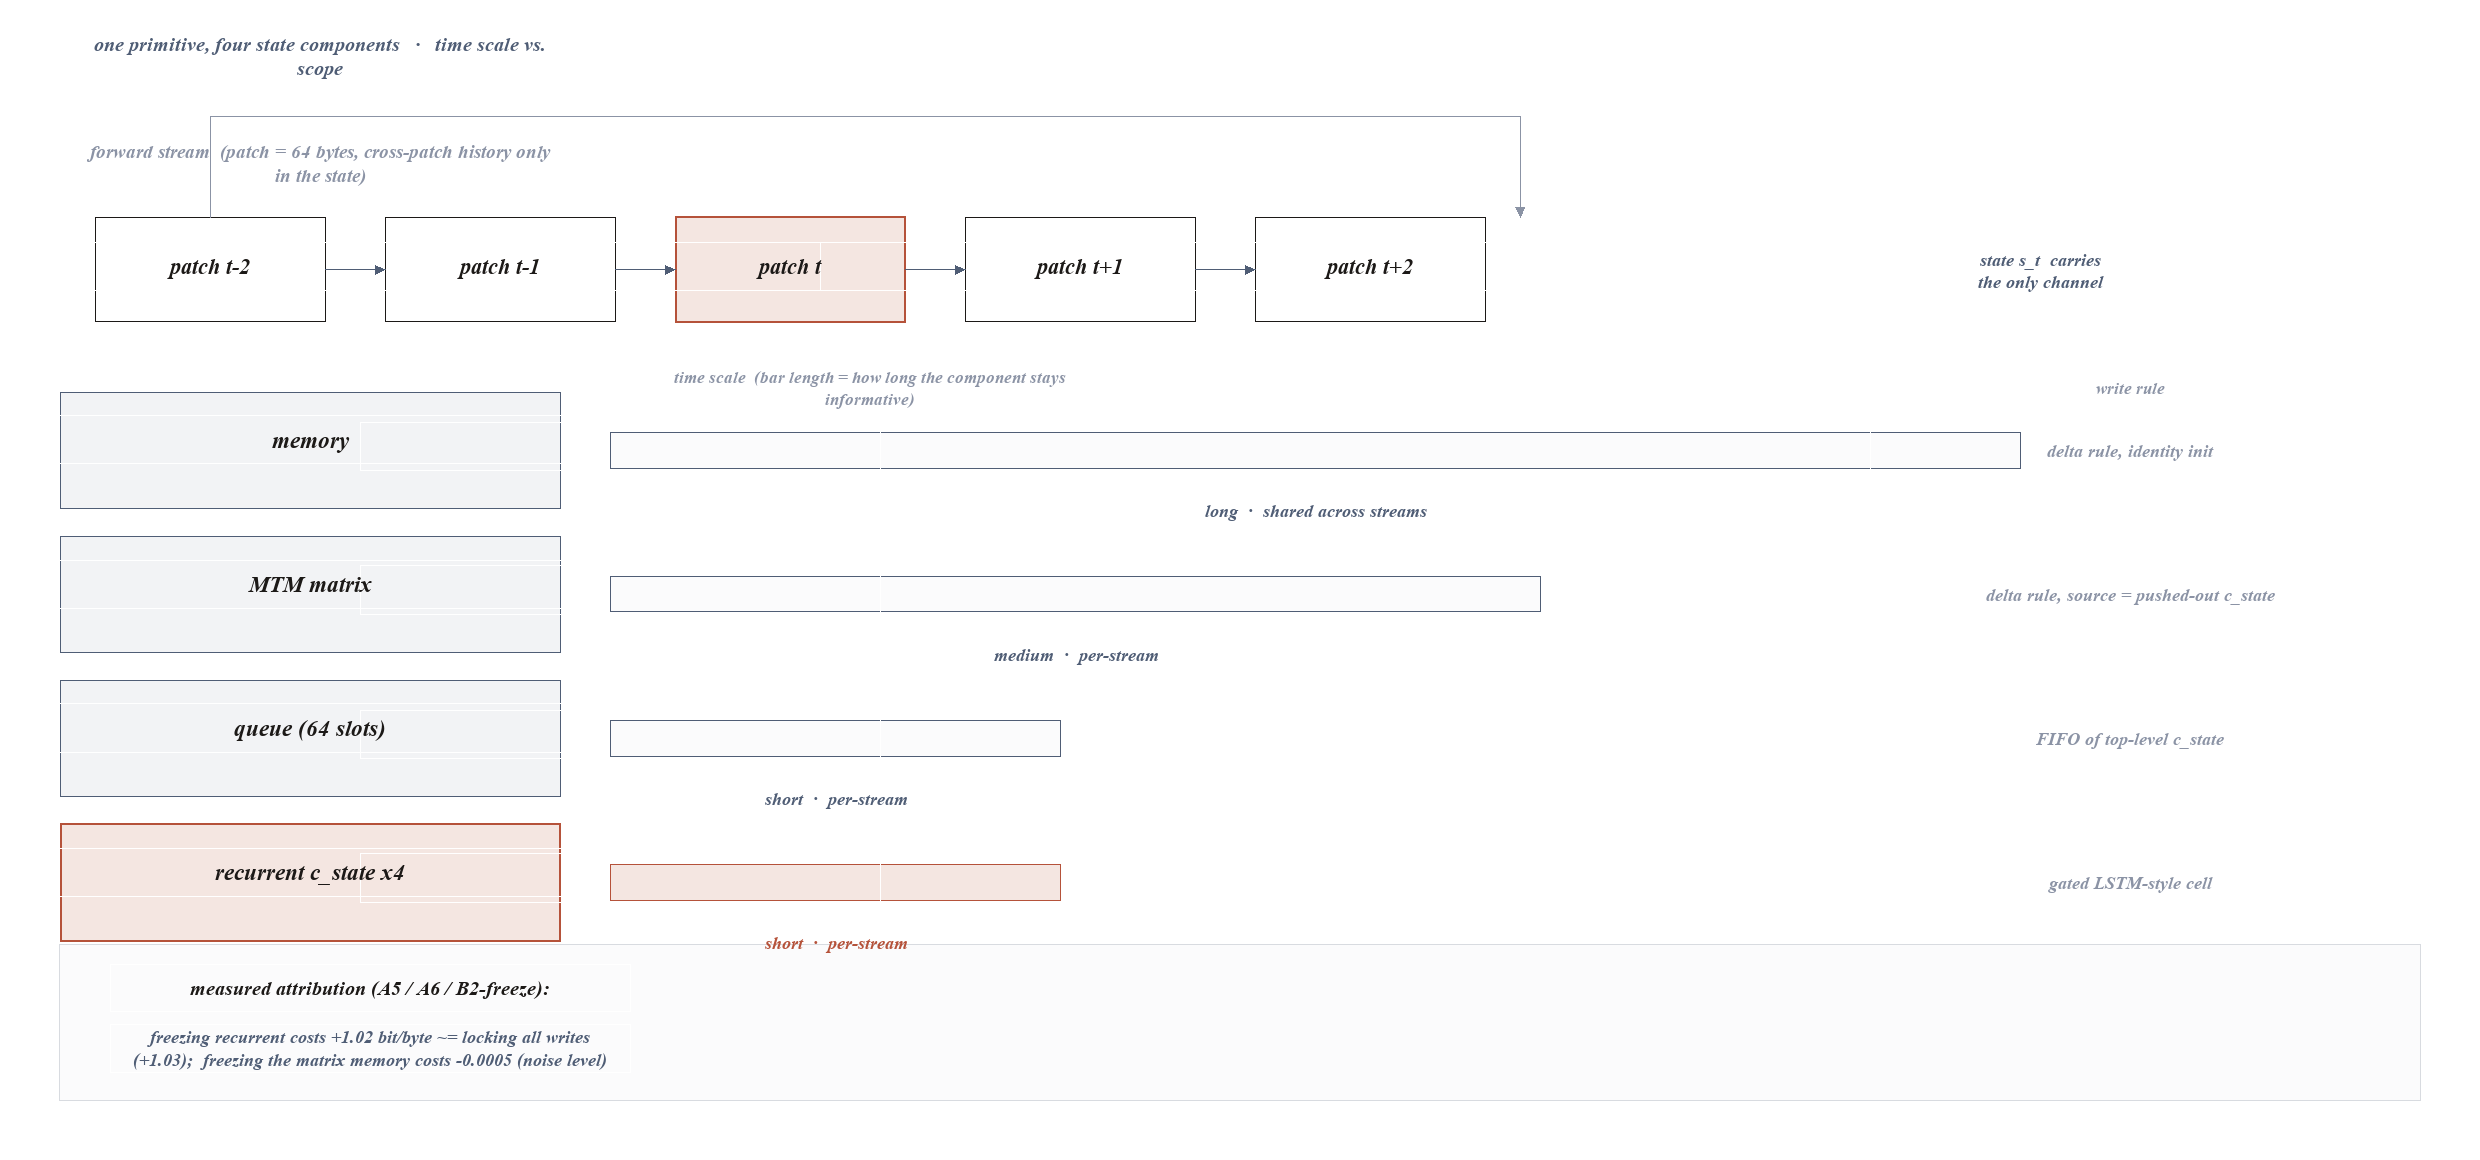
\includegraphics[width=\linewidth]{fig_state_scales.png}
\caption{四个状态分量的时间尺度与作用域（Visio 绘制，源文件 \texttt{figs/fig\_state\_scales.vsdx}）。
横条长度示意各分量「信息保持多久」的相对量级，右侧一列是写入规则；
底部给出本文实测的归属结论（A5/A6/B2-freeze 三组独立实验一致）。
注意「参数量最大的分量」并不等于「承担跨 patch 适应的分量」——这一区分由第 \ref{sec:s1} 章给出。}
\label{fig:state-scales}
\end{figure}

\textbf{作用域（按版本）。}v\_0d4 中\textbf{四个分量全部逐样本私有}——
\texttt{memory} 为每条序列独占的槽位（$[\mathrm{cap},\ldots]$，读取时按 $[:\mathrm{batch}]$ 切片），
训练提交不做跨流平均、跨卡不做同步（序列间零泄漏）。
本文检查点所属的 v\_0d3 则是「\texttt{memory} 一个共享、其余三个私有」的两族划分：
\texttt{memory} 写入后按流求均值、每 patch 一次跨卡 \texttt{all\_reduce}。
这个划分决定了「重置某个分量」实验（\S\ref{sec:s1-attr}）的语义——
在 v\_0d3 检查点上，重置 \texttt{memory} 相当于动跨样本的共享知识（本研究中等价于换回训练稳态快照），
重置其余三个只影响当前样本的上下文记忆；若换用 v\_0d4 检查点重跑，重置 \texttt{memory} 也将退化为
只影响当前样本的操作，\S\ref{sec:s1-attr} 的归因结论需要重新验证。
\textbf{本文所有实验都在 $\mathrm{batch}=1$ 上进行}，此时两版的 memory 读写逐位对应，
故推理侧结论不受该差异影响（\S\ref{sec:train}）。
\textbf{「多时间尺度」的分工叙述由实验支撑}，而不是凭结构空口断言：
本文在 \S\ref{sec:s1-attr} 用组件级重置与冻结给出分工的实测结果。

\textbf{原语。}四个分量是同一条 delta 规则在不同尺度上的实例（「一个原语、三个尺度」）：
读出 $\hat v = kM$，误差 $\Delta v = v - \hat v$，门控写入
\begin{equation}
M \leftarrow M + k^{\top}\!\left(g \cdot \Delta v\right),
\qquad g = \sigma(\cdot)\big/ \mathrm{eff\_seq\_len},
\label{eq:delta}
\end{equation}
随后读出 $qM + \text{因果分数} \cdot v_{\mathrm{dyn}}$。
式 \eqref{eq:delta} 是线性预测器的在线（岭）回归更新在秩空间中的实例，
$1/\mathrm{eff\_seq\_len}$ 缩放保证 patch 长度变化时写入量一致，门控 $g$ 使写入可以自适应减弱。

\subsection{状态的读写接口}\label{sec:model-io}

\textbf{两条前向路径：}\texttt{commit}（写入，$\mathit{lock\_mem}=\mathrm{false}$，状态正常更新）
与 \texttt{lock}（只读，$\mathit{lock\_mem}=\mathrm{true}$，状态原样直通）。
\textbf{本文所有实验的操纵旋钮都落在这两个接口上}——这是 \S\ref{sec:related-innovation} 中
「状态是微观实现、可以显式调整」的具体兑现。

\textbf{关键实现事实（受控设计的基础）：}$\mathit{lock\_mem}=\mathrm{true}$ 时四个状态分量原样直通，
因此\textbf{第一个 patch 的输出与正常前向逐位一致}——此时还没有发生任何写入；
从第二个 patch 起两者才因写入与否而分化，A2 测的就是这个分化量（\S\ref{sec:a2}）。

\textbf{推论。}状态因而是显式对象：前向返回新的状态对象而不原地修改，
所以它可以被整体读出、冻结、置换，也可以在同一份快照上并行地开出多个实验分支
（本文所有组件手术都是这个语义，见 \S\ref{sec:surgery}）。

\subsection{训练与检查点}\label{sec:train}

\textbf{状态不清零、跨批次连续（与 RNN/RWKV 的关键差别）。}
标准循环架构训练时状态从零初始化、一批读完即清零——单个状态最多跨一个样本的长度，
记忆跨不过样本边界。本文的模型\textbf{不按批次清空状态}：上一批结束时的状态直接续进下一批，
整条训练流是一条全局连续的流，状态的跨距不受样本长度限制。
batch 维被实现为若干条并行的永续数据流，\texttt{recurrent}/\texttt{queue}/\texttt{MTM} 逐流私有；
\texttt{memory} 在 v\_0d4 中同样逐流私有（每条流独占一个槽位，提交无跨流平均、跨卡无同步），
而本文检查点所属的 v\_0d3 为跨流共享（写入后按流平均，每 patch 一次跨卡 \texttt{all\_reduce}），
\texttt{chunk\_size}=192 条流。流数与 \texttt{bptt} 按版本配置：v\_0d3 为 $192$/$4$，
v\_0d4 的 MEDIUM 档改为 $1$/$16$。这正是「固定状态持续携带跨上下文信息」（S1）在训练侧成立的前提。

\textbf{记忆精度与门控初值（v\_0d4）。}记忆全程以 fp32 驻留（配置项 \texttt{mem\_dtype}，
可切 bf16 换显存，代价是小量级更新在 $|\mathrm{mem}|\!\sim\!1$ 处被舍入吸收）；
写入门控偏置初始化为 $-\ln 63\approx-4.14$，即 $\sigma(b)=1/64$，
使写入时间常数对齐 $64\times64=4096$ token 的队列视界（v\_0d3 为硬编码 $-6.0$）。

\textbf{优化与截断。}AdamW $+$ cosine 调度 $+$ 梯度裁剪 $1.0$，bf16 混合精度，
梯度窗口 \texttt{bptt}=4 个 patch（$4\times64=256$ token；本文检查点的 v\_0d3 配置，
v\_0d4 MEDIUM 档为 16 patch $=1024$ token）。
\textbf{截断窗口之外的长程信用只能经前向 delta 规则写入传递}——这是连到「持续学习」主张的关键设计点：
模型学到的不是「如何回传梯度到远处」，而是「如何在前向里把远处写进状态」。

\textbf{检查点与热启动。}训练收敛后状态达到稳态，检查点里保存的状态快照就作为评测的
\textbf{热启动}起点；若存档没有保存状态，则回退按空白处理。
存档格式随版本变化：v\_0d3 把共享 memory 存为顶层 \texttt{global\_memory} 字段（rank0 一份），
v\_0d4 把序列级 memory 放进各 rank 的 \texttt{runtime\_states}（rank 私有、全量落盘，
恢复时缺 memory 直接报错）——\textbf{两版存档互不兼容}。
本文使用 step $144{,}000/705{,}600$（约 20\% 训练进度）的中型检查点
\texttt{gridman\_medium\_v\_0d3\_pretrain}，取 batch$=1$ 切片的状态，
每次实验先克隆再跑——\textbf{状态跑一次就变}，不可复用同一对象，否则实验之间互相污染。
本文所有数字都建立在这个单一检查点上，因此\textbf{只做条件间比较}，绝对数值不可与外部模型对照（\S\ref{sec:limits}）。
